\documentclass{article}
\usepackage{color}
\usepackage[utf8]{inputenc}
\usepackage{amsmath}
\usepackage{listings}
\usepackage{graphicx}
\usepackage{enumerate}

\title{CIS 419/519: Homework 3}
\author{\{Your name here\}}
\date{}

\begin{document}

\maketitle
    Although the solutions are my own, I consulted with the following people while working on this homework: \{Names here\} \\
    
\section*{Neural Networks}
\subsection*{Feed Forward}
Plots:
\begin{center}
    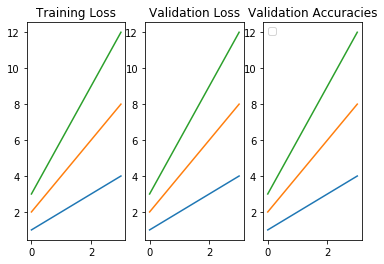
\includegraphics{example-plot.png}
\end{center}

\begin{center}
    \begin{tabular}{|c|c|}
        \hline
        Learning Rate & Final Validation Accuracy \\
        \hline
        0.0001 & \\
        0.00005 & \\
        0.00001 & \\
        \hline
    \end{tabular}
\end{center}
Learning rate with best validation accuracy: XXX.
The test accuracy of that model is YYY.

\subsection*{Convolutional}
Plots:
\begin{center}
    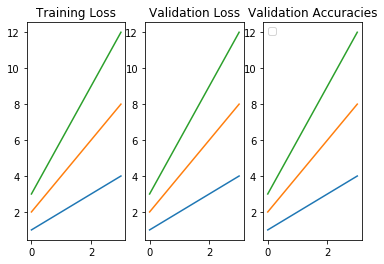
\includegraphics{example-plot.png}
\end{center}

\begin{center}
    \begin{tabular}{|c|c|}
        \hline
        Learning Rate & Final Validation Accuracy \\
        \hline
        0.01 & \\
        0.001 & \\
        0.0001 & \\
        \hline
    \end{tabular}
\end{center}
Learning rate with best validation accuracy: XXX.
The test accuracy of that model is YYY.

\section*{Boosting}
Fill in the boosting table below.
\begin{center}
        \begin{tabular}{|c|c||c|c|c|c||c|c|c|c|}
        \hline
          & & \multicolumn{4}{c||}{Hypothesis 1}
	  & \multicolumn{4}{c|}{Hypothesis 2} \\
          \cline{3-10}
          {\em i} & Label & $D_0$ & $f_1 \equiv $ & $f_2 \equiv $ & $h_1\equiv$ & $D_1$ &  $f_1 \equiv $ & $f_2 \equiv $ & $h_2 \equiv $ \\
          & & & [$x > {\color{red} b11} \;$] & [$y > {\color{red} c11}\;$] & [$\; {\color{red} d11} \;$] & & [$x > {\color{red} f11}\;$] & [$y > {\color{red} g11}\;$] & [$\;{\color{red} h11}\;$] \\
          
          & & & $\epsilon = {\color{red} b12}$ & $\epsilon = {\color{red} c12}$ & & & $\epsilon = {\color{red} f12}$ & $\epsilon = {\color{red} g12}$ & \\

          \tiny{(1)} & \tiny{(2)} & \tiny{(3)} & \tiny{(4)} &  \tiny{(5)} & \tiny{(6)} & \tiny{(7)} & \tiny{(8)} & \tiny{(9)} & \tiny{(10)}\\
          \hline \hline
          {\em 1} & $+$ & {\color{red} a1}; & {\color{red} b1}; & {\color{red} c1}; & {\color{red} d1}; & {\color{red} e1}; & {\color{red} f1}; & {\color{red} g1}; & {\color{red} h1};  \\
          \hline
          {\em 2} & $+$ & {\color{red} a2}; & {\color{red} b2}; & {\color{red} c2}; & {\color{red} d2}; & {\color{red} e2}; & {\color{red} f2}; & {\color{red} g2}; & {\color{red} h2};  \\
          \hline
          {\em 3} & $+$ & {\color{red} a3}; & {\color{red} b3}; & {\color{red} c3}; & {\color{red} d3}; & {\color{red} e3}; & {\color{red} f3}; & {\color{red} g3}; & {\color{red} h3}; \\
          \hline
          {\em 4} & $+$ & {\color{red} a4}; & {\color{red} b4}; & {\color{red} c4}; & {\color{red} d4}; & {\color{red} e4}; & {\color{red} f4}; & {\color{red} g4}; & {\color{red} h4}; \\
          \hline
          {\em 5} & $+$ & {\color{red} a5}; & {\color{red} b5}; & {\color{red} c5}; & {\color{red} d5}; & {\color{red} e5}; & {\color{red} f5}; & {\color{red} g5}; & {\color{red} h5}; \\
          \hline
          {\em 6} & $-$ & {\color{red} a6}; & {\color{red} b6}; & {\color{red} c6}; & {\color{red} d6}; & {\color{red} e6}; & {\color{red} f6}; & {\color{red} g6}; & {\color{red} h6}; \\
          \hline
          {\em 7} & $-$ & {\color{red} a7}; & {\color{red} b7}; & {\color{red} c7}; & {\color{red} d7}; & {\color{red} e7}; & {\color{red} f7}; & {\color{red} g7}; & {\color{red} h7}; \\
          \hline
          {\em 8} & $-$ & {\color{red} a8}; & {\color{red} b8}; & {\color{red} c8}; & {\color{red} d8}; & {\color{red} e8}; & {\color{red} f8}; & {\color{red} g8}; & {\color{red} h8}; \\
          \hline
          {\em 9} & $-$ & {\color{red} a9}; & {\color{red} b9}; & {\color{red} c9}; & {\color{red} d9}; & {\color{red} e9}; & {\color{red} f9}; & {\color{red} g9}; & {\color{red} h9}; \\
          \hline
          {\em 10} & $-$ & {\color{red} a10}; & {\color{red} b10}; & {\color{red} c10}; & {\color{red} d10}; & {\color{red} e10}; & {\color{red} f10}; & {\color{red} g10}; & {\color{red} h1}; \\
          \hline
        \end{tabular}
\end{center}
The final hypothesis is
\begin{equation}
    H_\textrm{final} = ...
\end{equation}

\section*{SVMs}
\begin{enumerate}[(a)]
    \item \begin{enumerate}[1.]
        \item $\mathbf{w} = [a, b]$, $\theta = ...$
        \item $\mathbf{w} = [a, b]$, $\theta = ...$
        Explanation for how you reached this answer...
    \end{enumerate}
    \item \begin{enumerate}[1.]
        \item $I = $
        \item Write $\alpha = $ for each $\alpha$
        \item Objective function value:
    \end{enumerate}
    \item Explanation of the different values for $C$
\end{enumerate}

\end{document}